\documentclass[review]{elsarticle}
\usepackage{lineno,hyperref}
\usepackage{subcaption}
\usepackage{siunitx}
\usepackage{booktabs}
\usepackage{graphicx}
\usepackage{appendix}
\usepackage{amsmath} 
\usepackage[hang,flushmargin]{footmisc} 
\usepackage{xcolor}
\usepackage{float}
\usepackage{array,multirow}
\usepackage{hyperref}
\usepackage{setspace}
\usepackage{stmaryrd}
\usepackage{enumitem}
\usepackage{rotating}
\usepackage{adjustbox}
\usepackage{array}
\usepackage{booktabs}
\usepackage{xcolor,colortbl}
\usepackage{amsmath} 
\usepackage{amsfonts} 
\usepackage{amssymb}
\usepackage{makecell}
\usepackage{amsmath}
\usepackage{nicefrac}
\usepackage{todonotes}
\usepackage{multirow}
\modulolinenumbers[1]
\usepackage{lineno}
\usepackage{tikz}

%\usepackage[final]{changes}
\usepackage{changes}
\usepackage[ruled,vlined,linesnumbered,lined,boxed,commentsnumbered]{algorithm2e}
\newcommand\mycommfont[1]{\footnotesize\ttfamily\textcolor{blue}{#1}}
\SetCommentSty{mycommfont}
\newcommand{\BREAK}{\STATE \algorithmicbreak}
\modulolinenumbers[1]
\setlength{\parindent}{0em}
\journal{Applied Energy}
\bibliographystyle{elsarticle-num}

\begin{document}
\begin{frontmatter}

%\title{Justice in decarbonizing heating systems consistent with the Paris Climate Agreement: subsidy balance between landlords and tenants at the multi-apartment building level}
\title{Cost-optimal and socially balanced subsidization strategy incentivizing a just heating system decarbonization at the building level}
\author[1]{Sebastian Zwickl-Bernhard\corref{cor1}}
\ead{zwickl@eeg.tuwien.ac.at}
\author[1]{Hans Auer}
\author[1]{Antonia Golab}
\cortext[cor1]{Corresponding author}
\address[1]{Energy Economics Group (EEG), Technische Universität Wien, Gusshausstrasse 25-29/E370-3, 1040 Wien, Austria}

\begin{abstract}

\end{abstract}

\begin{keyword}
	
\end{keyword}
\end{frontmatter}

\newpage
\todo{Thursday 28.10.2021}
\section*{Nomenclature}
\begin{center}
	\renewcommand{\arraystretch}{1.1}
	\centering
	\small
	\begin{tabular}{lm{8cm}r}
		Type & Description & Unit\\
		\hline
		Set and index & & \\
		\hline
		
		{$y \in \mathcal{Y}=\{1,\ldots,Y\}$} & Years, index by $y$\\
		{$m \in \mathcal{M}=\{1,\ldots,M\}$} & Months, index by $m$\\
		
		\hline
		Decision variables\\
		\hline
		{$inv_{grant}$} & Landlord's investment grants & \SI{}{EUR}\\
		{$sub_{heat,y,m}$} & Tenant's heating costs subsidy in $y$ and $m$ & \SI{}{EUR}\\
		{$q_{init,y,m}$} & Heat demand supplied by the initial heating system & \SI{}{kWh}\\
		{$q_{alt,y,m}$} & Heat demand supplied by the heating system alternative & \SI{}{kWh}\\
		{$\Pi_{alt}$} & Newly installed heating system alternative capacity & \SI{}{kW}\\
		{$r_{y,m}$} & Rent charge adjustment in $y$ and $m$ & \SI{}{EUR\per m^2}\\
		\hline
		Parameters\\
		\hline
		{$n_{ten}$} & Number of tenants & \SI{}{1}\\
		{$i$} & Interest rate & \SI{}{\%}\\
		{$q_{load,y,m}$} & Total heat demand in $y$ and $m$ & \SI{}{kWh}\\
		{$\alpha_{m}$} & Ratio between total heat demand and peak load in $m$ & \SI{}{1}\\
		{$c_{alt,hs}$} & Specific heating system alternative investment costs & \SI{}{EUR \per kW}\\
		{$c_{alt,con}$} & Heating system alternative construction costs & \SI{}{EUR}\\
		{$\bar{r}$} & Initial rent price & \SI{}{EUR \per m^2}\\
		{$a$} & Rented area per tenant & \SI{}{m^2}\\
		{$p_{init,y}$} & Energy price fueling the initial heating system & \SI{}{EUR \per kWh}\\
		{$p_{alt,y,m}$} & Energy price fueling the heating system alternative & \SI{}{EUR \per kWh}\\
		\hline
	\end{tabular}
\end{center}
\newpage

\section{Introduction}
The recently published "Fit for 55" package \cite{european_commission_european_2019} by the European Commission outlines the pathway until 2030 to reduce greenhouse gas emissions by \SI{55}{\%} compared to 1990 in the Europe Union (EU). With an eye on the therein described energy policy recommendations, undisputedly, massive efforts across sectors are necessary to enable a sustainable transformation of the energy system (see also in \cite{korkmaz2020comparison}). At the same time, there is a need for energy justice complying with the manner of "no one left behind" \cite{sovacool2019decarbonization}. Against this background, the residential building sector calls for particular attention. There are at least three reasons for this: (i) high shares of fossil fuels in the provision of heat service needs (and increasingly cold services as well), (ii) inefficient ways of delivering the heat demand caused by low standards of both building stock quality and heating devices, (iii) complex building ownership structures and finally the landlord/tenants nexus in rented apartments or dwellings.\vspace{0.5cm}

In fact, buildings are responsible for \SI{40}{\%} of EU energy consumption and \SI{36}{\%} of the greenhouse gas emissions in $2021$. Moreover, the European Commission states that \SI{75}{\%} of EU's buildings are energy inefficient. The essential factor to improve these indicators is building retrofitting. Passive renovation measures can already make a significant contribution, as \SI{35}{\%} of EU's buildings are older than \SI{50}{} years. However, retrofitting alone will not be sufficient for a deep decarbonization of the European building stock. Rather, it is necessary to increase the current renovation rate of \SI{1}{\% \per year} \cite{eurocombuildings2021}. Thus, the share of passive (e.g., building skin insulation improvements) alongside active renovation (e.g., heating system change) measures needs to be increased rapidly to be compliant with European climate plans such as the abovementioned Fit for 55 package. Indeed, European decarbonization scenarios assume a much higher renovation rate up to \SI{3}{\%} per year in order to achieve climate neutrality \cite{korkmaz2020comparison}. To increase this rate, most scientific literature findings suggest federal financial incentives since renovation measures do not achieve economic viability under current market environments in the EU (see, e.g., Fina et al. \cite{fina2019profitability}, Weber and Wolff \cite{weber2018energy}, and Kumbaroğlu and Madlener \cite{kumbarouglu2012evaluation}).\vspace{0.5cm}

We have already seen in the last decades how federal financial incentives have led to massive market penetration of renewable energy technologies. For example, in recent years solar photovoltaic (PV) has flooded the electricity markets driven by public monetary subsidies such as feed-in tariff programs \cite{hoppmann2014compulsive}. In addition, significant cost reductions were achieved due to efficiency improvements and economies of scale \cite{haas2011historical}. In principle, there are good reasons to think that one can learn from the diffusion pathway of solar PV and related experiences. Nevertheless, two aspects are crucial in this context that has received too little attention in the past. First that the public monetary diffusion of renewable energy has to be accompanied by measures ensuring energy efficiency and thus energy savings. Recently, Poponi et al. \cite{poponi2021subsidisation} conducted a subsidization cost analysis of solar PV in Italy. where they concluded that public monetary support strategies are cost-ineffective policy instruments if energy efficiency investments are ignored. And secondly, that the support must be socially balanced in a society with and without private ownership. In the energy transition process, this is essential for both renewable generation and demand sector.\vspace{0.5cm}

The scope of this paper aims at exploring how to deal with one of the "hot potatos" on the road to a sustainable society: namely, to trigger investments for deep decarbonization of the rented residential building sector in terms of heating system change and passive retrofitting. The focus is put on multi-apartment buildings in urban areas that are often heated by natural gas-based heating systems. Moreover, the frequently occurring ownership structure within the building with a single landlord (building owner) and numerous tenants plays a key role in the analysis as this is a generally crucial relationship. Typically, a building's landlord is the investment decision-maker in terms of potential (active and passive) energy efficiency measures but is not affected its decision process by an increasing CO\textsubscript{2} price as the most significant determining parameter of deep decarbonization. On the contrary, the tenants are at the mercy of the future CO\textsubscript{2} development and have no decision-making power to counteract it, e.g., by changing the heating system.\vspace{0.5cm}

Against this background, the core objective of this work is to set up a cost-optimal and socially balanced subsidization strategy for a multi-apartment building to trigger investments in a sustainable heat supply. A public authority (governance) incentivizes the replacement of the initial natural gas-based heating system toward a sustainable alternative along with building renovation measures (accompanied by reduced heat demand) by monetary support to the landlord and the tenants. Monetary support can be direct payments in the form of an investment grant for the landlord or a subsidy payment for the tenant. Besides, the owner (i.e., landlord) can also be indirectly financially supported by allowing a rent adjustment as the building is refurbished. Social balance is defined at the building level from a monetary perspective using the net present value of the governance's total payments for the building's owner and the tenants.\vspace{0.5cm}

The method applied is the development of a linear optimization model. Thereby, the objective function is to minimize the governance's net present value of financial support over time. The landlord's and tenants' strategy to minimize the individual total costs is considered by tailor-made constraints in the modeling framework. The generalized formulation of the model allows to investigate different building types and categorizes (e.g., size and number of tenants, building efficiency, initial rent price, etc.). This can be helpful to analyse different building stocks.\vspace{0.5cm}

The numerical example examined is an old multi-apartment building with a single owner (landlord) and 30 units (tenants). The partially renovated building is located in an urban area (Vienna, Austria) and initially heated by individual gas heating systems at the unit's level. The decarbonization of the heat supply can be achieved by two different investment options, namely, a connection to the district heating network or an implementation of an air-sourced heat pump system on building level.\vspace{0.5cm}

The paper is organized as follows. Section \ref{stateoftheart} summarizes the current state-of-the-art in literature and outlines the own contribution of this work beyond existing research. Section \ref{methodology} presents the materials and methods developed in this work including the mathematical formulation of the model, scenarios, description of numerical example description and model validation. Section \ref{results} presents the results of this work, including sensitivity analyses of key determining parameters. Section \ref{conclusions} discusses the results, concludes the work, and outlines possible future research.
\newpage
\section{State-of-the-art and progress beyond}\label{stateoftheart}
This section aims to provide an overview of relevant scientific contributions with respect to this paper's scope. Explicitly not part of the literature review is the already widely discussed topic of sharing renewable energy generation and related peer-to-peer innovations in the light of energy communities. A general study comprehensively dealing with the sharing economy is provided by Codagnone and Martens \cite{codagnone2016scoping}. The reviews from Sousa et al. \cite{sousa2019peer} and Koirala et al. \cite{koirala2016energetic} go into even more depth and with resepect to peer-to-peer energy sharing and energy communities. Also the authors' literature review of this paper in \cite{zwickl2021open} provides a comprehensive review of energy sharing on the local level.\vspace{0.5cm}

Against this background, the focus here lies on three different dimensions without claiming to be absolutely complete in each case. The first dimension is the decarbonization of heating and cooling systems from a system analysis perspective and is described in Section \ref{aspect1}. The second dimension deals with the increasingly importance of justice in the energy system transition and is presented in Section \ref{aspect2}. The third dimension is dedicated to the trade-offs analysis of investment decisions into renewable energy technologies including realted contracting business cases and is discussed in Section \ref{aspect3}. The choice of these focal points, as well as the explicit exclusion of the mentioned topics, are deliberately chosen in order to reflect the DNA of the analysis. 

\subsection{Decarbonizing the provision of heating service needs}\label{aspect1}
The insights obtained from various scientific studies allow us to see the big picture of a decarbonized heating and cooling sector. A fundamental change of the energy carrier mix, alongside a significant efficiency increase, is necessary for a sustainable heating and cooling service need supply. For example, Connolly et al. \cite{connolly2014heat} provide in their study such a strategy and present a decarbonization roadmap for the European heating sector. They propose a new sustainable heat strategy that is based on changes on the demand-side and supply-side. In addition to significant heat savings, integrating sustainable heat sources into centralized heat networks (or district heating networks) and electrifying heat supply (e.g., heat pump) are suggested to achieve a low-carbon heating sector. Seyboth et al. \cite{seyboth2008recognising} focus in their study on supportive energy policy recommendations to enhance the deployment of renewable energy heating and cooling technologies. In particular, this means the integration of renewable sources such as solar, geothermal, and biomass into heating and cooling systems.\vspace{0.5cm}

In general, the sustainable heat source or heat generation technology that is ultimately implemented/used at the end-user levels depends on a number of factors. Among these, geographical and spatial characteristics (e.g., availability of heat network infrastructure, building construction features, outdoor temperature, etc.), in particular, play a crucial role. Su et al. \cite{su2018heating} deal in their study with optimal sustainable heating system alternatives with a special focus on local geographical features of the application site. Their results show that there might not be a one-fits-all solution if decarbonizing local heating systems. However, certain trends are very much emerging in their findings, which can also be confirmed by further case studies. Renewable-fed district heating networks have significant potential to supply heat demand in urban areas. This is exemplarily also shown by the results of Popovski et al. \cite{popovski2018technical}. They state that from a socio-economic perspective, district heating networks with excess heat are the most favorable supply option in densely populated areas. Lake et al. \cite{lake2017review} present a comprehensive review of district heating and cooling systems. They analyze among others the economic feasibility and system identification based on primary energy sources of centralized heating and cooling networks. Rama et al. \cite{rama2018introduction} study the optimal combination of different sustainable heating alternatives.In particular, they show how heat pumps and solarthermal can assist district heating networks. There exist also other alternatives. Sopha et al. \cite{sopha2011exploring} focus in their study on the potential of wood-pellet in Norway, a country with high shares of district heating-based heat supply. They use an agent-based model to identify energy policy options supporting the uptake of such sustainable heating systems. The authors conclude that a stable financial support (i.e., stable wood-pellet price) has the highest impact on the transition of wood-pellet. We refer to Section \ref{aspect3} in this context for a detailed discussion of financial incentives for renewable energy technologies in the heating sector.\vspace{0.5cm}

In any case, there is a need for sustainable alternatives to district heating. Either to complement existing district heating networks in a high-efficient way (e.g., \cite{rama2018introduction} and \cite{sopha2011exploring}) and/or because to compensate non-existing networks in the future. Popovski et al. \cite{popovski2018technical} identify the electrification of the heat supply using heat pumps with photovoltaics as the most cost-competitive alternative from a socio-economic perspective. Leibowicz et al. \cite{leibowicz2018optimal} also show end-use electrification as an optimal strategy for the decarbonization of the heating sector. However, the authors state that the electrification using heat pumps for example only makes sense in combination with building thermal efficiency improvements.\vspace{0.5cm}

In order to emphasize the importance of building renovation measures, we dedicate this concluding paragraph the corresponding literature. In particular, we select papers focusing on the impact of different retorfitting measures on sustainable heating system alternatives. However, we do not differentiate here in detail between different types of retrofitting measures (e.g., purely passive, passive, active, etc.) and refer in this context to the comprehensive literature review of Fina et al. in \cite{fina2019profitability}. Ma et al. \cite{ma2012existing} provide an extensive literature and state-of-the-art analysis of retrofitting focusing on existing buildings. Vieites et al. \cite{vieites2015european} elaborate in this context of European initiatives improving  the energy efficiency in existing and old (historic) buildings. Recently, Weinberger et al. \cite{weinberger2021investigating} investigate the impact of retrofitting on district heating networks. Fina et al. \cite{fina2019profitability} put their focus on the profitability of retrofitting of multi-apartment buildings with special consideration of different heating systems. They thoroughly study the implementation of the combination of building-attached/integrated photovoltaics supporting sustainable heating systems. Their results show how (passive) retrofitting measures result in a reduction of the required installed heating system capacity. However, the energy cost reduction achieved from higher building standards are not able to compensate the initial passive renovation investment costs. They conclude that latter significantly depend on the development of the CO\textsubscript{2} price and the assumptions of end-user investment grants as well as subsidies. We again take up these findings associated with financial support in Section \ref{aspect3}

\subsection{Justice in energy systems: fair and socially balanced sustainable energy transition}\label{aspect2}
The issue of justice in energy systems is addressed in various studies. According to them, a key part of achieving climate targets is to ensure that no one is left behind in the climate action. More generally, the three energy justice tenets are distributive, recognition, and procedural\footnote{In some works, restorative and cosmopolitan justice are also mentioned in this context. See, exemplarily in \cite{oxfordjustice2021}.}. Recently, these are comprehensively discussed and reviewed by Pellegrini et al. \cite{pellegrini2020energy}. Considering this work's scope, we put our focus on procedural justice, as it represents measures that reduce potential barriers to new clean energy investments \cite{oxfordjustice2021}.\vspace{0.5cm}

Generally speaking, dealing with just sustainable energy systems is a monumental task and seems to be very challenging to be generalized. However, studies focusing on certain local regions are likely to be the most promising approach. Recently, van Bommel and Höffken conducted a review study focusing on energy justice at the European community level \cite{van2021energy}. Besides that, Lacey-Barnacle et al. \cite{lacey2020energy} focus in their study on energy justice in developing countries. Coming back to this paper's content and spatial scope, Mundaca et al. \cite{mundaca2018successful} propose two local European case studies in Germany and Denmark investigating local energy transition from an energy justice perspective. Their findings are in line with those from Jenkins et al. \cite{jenkins2018humanizing} showing that energy justice and transitions framework can be combined and achieved simultaneously. However, Hiteva and Soacool \cite{hiteva2017harnessing} conclude from a business model perspective that energy justice may be realized through market principles but not through the market alone. We continue discussing this point in Section \ref{aspect3} when dealing with necessary (financial) incentives that foster the sustainable energy transition. \vspace{0.5cm} 

Recently, Hanke et al. \cite{hanke2021renewable} investigate renewable energy communities and their capability to deliver energy justice. They explore insights from 71 European cases and highlight the necessity of distributing affordable energy to vulnerable households. Furthermore, it is necessary to focus in this regard on low-income households. Exemplarily, Xu and Chen \cite{xu2019energy} propose on the basis of their generated results that low-income households need tailored assistance to ensure energy justice. In particular, they demonstrate that low-income households are renters and thus have fewer energy efficiency appliances. Sovacool et al. \cite{sovacool2019temporality} heat in the same direction and discuss the special difficulties for households without the capital for sustainable energy investments and for those that do not own their own home such as renters. Moreover, renters also often have higher residential heating energy use intensity, an energy efficiency proxy \cite{reames2016targeting}. In this context, Greene \cite{greene2011uncertainty} discussed the so-called “efficiency gap” or “energy paradox". He showed that consumers have a bias leading to undervaluation of future energy savings in relation to their expected value. The main reasons are a combination of two aspects, namely, an uncertainty regarding the net value of future fuel savings and the loss aversion of typical consumers. Filling the abovementioned efficiency gap is crucial in order to achieve both the energy transition and energy justice. Sovacool et al. \cite{sovacool2019decarbonization} show that unfolding the energy transition result in deeper injustices investigating four different low-carbon transitions.

\subsection{Overnight investments versus net present value}\label{aspect3}
In particular, this concluding section is about looking at different renewable energy promotion instruments focusing on the heating sector. However, in some places, we refer to literature that deals in detail with the electricity sector. We consider this to be useful for the reader, to show the parallels and differences between the two sectors through comparison. Connor et al. \cite{connor2013devising} provide a fundamental review paper investigating a wide range of policy options that can support the deployment of renewable heat technologies. Masini and Menichetti \cite{masini2012impact} state that despite numerous energy policies implemented to promote renewable energy technologies, the penetration of these remains below expectations. They identify as one main key a lack of appropriate financing investment incentives. Public (financial) incentives are often seen as the most appropriate and efficient measures to fill this gap. Reuter et al. \cite{reuter2012renewable} compare different policy instruments, ranging from feed-in tariffs to investment subsidies, tax credits, portfolio requirements, and certificate systems. While focusing on companies and their willingness for renewable energy technology investments in the electricity sector, they conclude that feed-in tariffs are an effective means promoting these investments\footnote{Zhou et al. \cite{zhou2011designing} provide a study dealing with the effectiveness of public financial incentives. The authors define effectiveness/efficiency as the amount of intervention (e.g., taxes collected, subsidies paid, etc.) to achieve a policy goal. Here, it is essentially the electricity sector that is being studied.}. Similar results also can be found in the study from Couture and Gagnon \cite{couture2010analysis}. Nevertheless, the two latter studies only investigate the deployment of renewable energy technologies in the electricity sector and not in the heating sector.\vspace{0.5cm} 

Building on these literature findings, however, it is of particular importance to differentiate between renewable energy technology investments from companies and private end-customers and households. In contrast to companies, private households are incentivized more effectively by investment grants to invest in renewable energy technologies \cite{roth2020impact}. This distinction and targeted adjustment of public financial incentives are important since private investment is a key driver of the diffusion of renewable energy technologies \cite{wustenhagen2012strategic}. {\O}stergaard et al. \cite{ostergaard2019costs} investigate the investment costs of households to prepare existing buildings for high-efficient and sustainable heating systems. Their results show that customer investments require financial incentives and are required to be motivated economically\footnote{In particular, {\O}stergaard et al. \cite{ostergaard2019costs} show that the investment into an expansion of an existing low-temperature district heating network can be seen significantly differently. For example, a heat supply company achieves economic viability with the investment considering the potential of newly supplied heat demand in the area. However, it is not guaranteed that new consumers aim to be connected to the network since their investment profitability is highly uncertain due to high connection costs and low heat energy price savings.}. In this context, the role of an increasing CO\textsubscript{2} price should also be interpreted with particular circumspection. Although, in general, the literature sees carbon pricing as the most important measure speeding up the sustainable energy system transition (see, for example, Nägeli et al. \cite{nageli2020policies} focusing on the impact of carbon pricing on the residential building sector). However, this does not solve the inherent problem of differential ownership in the residential sector (i.e., landlords and tenants/renters). It is, therefore, only logical that Hecher et al. \cite{hecher2017trigger} focus in their work on the decision-making processes regarding sustainable heating system investments of homeowners. Therefore, there is a gap in the literature dedicated precisely to a heating system change in the residential sector, not neglecting the different ownerships.\vspace{0.5cm} 

We conclude this section with the topic of energy and heat contracting business models and explicitly aim to give only a small overview, as contracting business models themselves are not part of the paper's main scope. A comparative review of municipal energy business models in different countries is given by Brinker and Satchwell \cite{brinker2020comparative}. Kindström and Ottosson \cite{kindstrom2016local} analyze local and regional energy companies offering energy services and conclude that most many of these are experiencing difficulties on the market. One reason is, as Fine et al. state, that the contracting framework itself decreases the economic viability since the contractor business companies (third party) aim to gain profit (i.e., contractor's interest rate). Suhonen and Okkonen \cite{suhonen2013energy} conduct an analysis of energy service companies in the residential heating sector and show a wide-ranging set of barriers of such business models. Moreover, the results of their Finnish case study reveal that this kind of contracting business model is unattractive and not profitable. Brown \cite{brown2018business} investigates business models for residential retrofit in the United Kingdom and the European Union. Fina et al. \cite{fina2020profitability} study the profitability of contracting business cases for shared photovoltaic generation and renovation measures in a residential multi-apartment building. Their results indicate that the profitability of (passive) building renovation measures significantly depends on the carbon price. However, the difficulties of high carbon prices are already addressed above and in the novelties of this work in the next section. Furthermore, Fina et al. focus explicitly in their study on building owners and neglect different ownership relationships.  

\subsection{Progress beyond state-of-the-art}\label{novelties}
Based on the abovementioned literature review, the scientific contribution and the novelties of this paper can be summarized as follows:
\begin{itemize}
	\item A sustainable heating system change with a focus on the efficient provision of heat service needs at the multi-apartment building is carried out, emphasizing the ownership structure of the building and related financial interests of the building owner and the different tenants/renters. In particular, this addresses one of the hot potatoes of deep decarbonization strategies, namely, the residential heating sector with tenants who cannot change the heating system on their own due to missing ownership, and therefore extra attention need. The sustainable heating system alternative is financially incentivized by a federal subsidy strategy considering monetary justice between the landlord and the tenants. 
	\item The developed analytical framework determines a cost-optimal and socially balanced subsidization strategy from the governance incentivzing a just heating system decarbonization at the building level. Especially, the optimization model allows a quantitative analysis of justice in low-carbon residential heating sector including the agent's specific monetary interests and the ownership structure within a building. Thus, this work focus on the trade-off analysis between the governance, landlord and tenants.
	\item The sensitivity analysis of sharing carbon-related energy costs between the building owner and tenants on the one hand, and linking the governance's strategy directly to building retrofitting measures, on the other hand, represent substantial innovations in the field of research for decarbonizing the existing building stock with landlord and tenants relations. The insights gained in this context help build a better understanding of decarbonizing the existing (rented) building stock. Even more, this work may contribute to rapidly increasing the renovation rate, often seen as a key for a high-efficient and decarbonized residential sector. 
\end{itemize}
\newpage
\section{Materials and methods}\label{methodology}
This section explains the methodology and the optimization model developed in this work. The section starts with an introduction and overview of the model in Section \ref{met:intro}. This is followed by a detailed description of the mathematical formulation in Section \ref{met:formulas}. A case study description and empirical settings are presented in Section \ref{met:empirical}, and model validation is shown in Section \ref{met:validate}.

\subsection{Introduction and overview of the model}\label{met:intro}

\begin{figure}[h]
	\centering
	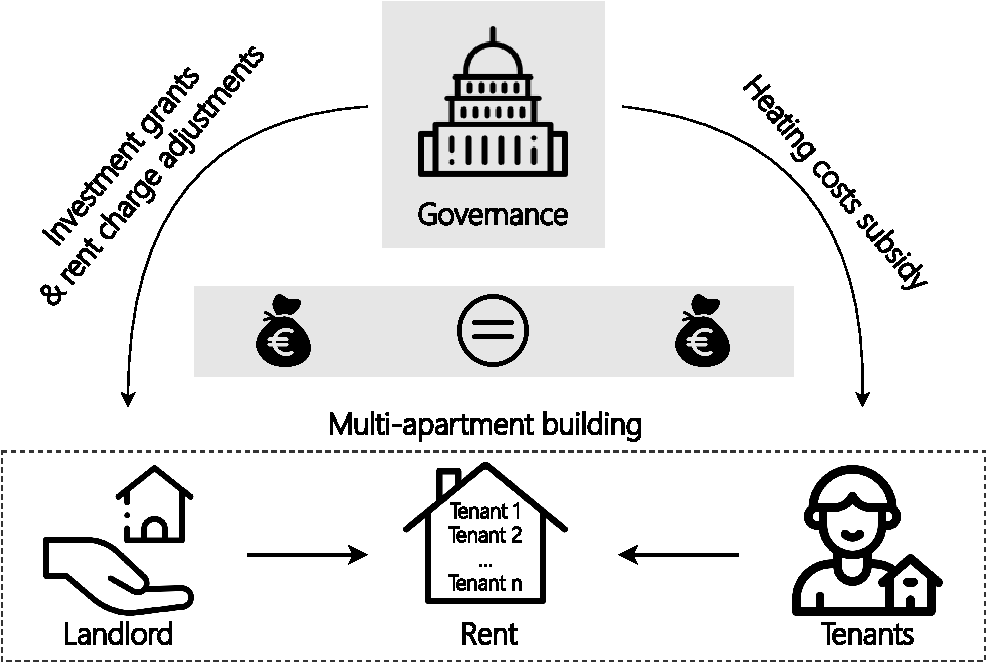
\includegraphics[width=0.9\linewidth]{figures/3_Methodology/Sketch.pdf}
	\caption{}
	\label{fig:methodology}
\end{figure}





\subsection{Mathematical formulation of the model}\label{met:formulas}

\paragraph{Objective function}
The objective function of the model is to minimize the governance's total costs for investment grants and subsidies. Therefore, the objective function can be written as follows: 
\begin{align}\label{objective}
\underset{x}{\mathrm{min~}} \underbrace{inv_{grant}}_\text{landlord} + \sum_{y} \sum_{m} n_{ten} \cdot \frac{1}{(1+i_g)^y} \cdot \underbrace{sub_{heat,y,m}}_\text{tenant}
\end{align}

where $inv_{grant}$ is the investment grant for the landlord and $sub_{heat,y,m}$ the tenant's subsidy for the heating costs in year $y$ and month $m$. In addition, $n_{ten}$ is the number of tenants\footnote{It is assumed that the multi-apartment building consists of $n_{ten}$ equal tenants. This is a simplification, however, in this paper we do not focus on the socially balanced between tenants, but on that between the landlord and the tenants.} and $i_g$ the governance's interest rate. The model's decision variables are included in the decision variable vector $x$.

\paragraph{Decision variables}
In order to improve the readability of the section, we explicitly list all the decision variables of the model using $x$
\begin{align}
\b{$x$}=[inv_{grant}, sub_{heat,y,m}, q_{init,y,m}, q_{alt,y,m}, \Pi_{alt}, r_{y,m}]
\end{align}

where $q_{init,y,m}$ is the quantity of heat demand supplied by the initial heating system using conventional fuels and $q_{alt,y,m}$ using the sustainable heating system alternative in $y$ and $m$. $\Pi_{alt}$ is the capacity of the newly installed heating system alternative and $r_{y,m}$ the rent charge in $y$ and $m$.

\paragraph{Constraints} Equation \ref{c:demand} describes the load satisfaction in each time steps (year and month) 
\begin{align}\label{c:demand}
q_{load,y,m} \leq q_{init,y,m} + q_{alt,y,m} \quad :\forall y,m
\end{align}

where $q_{load,y,m}$ is the total heat demand of the multi-apartment building. Equation \ref{c:capacity} defines the minimum required newly installed capacity of the heating system alternative
\begin{align}\label{c:capacity}
\alpha_{m} \cdot q_{alt,y,m} \leq \Pi_{alt} \quad :\forall y,m
\end{align}

where $\alpha_{m}$ is a factor that transforms the amount of monthly heat demand to the corresponding peak demand (i.e., monthly heating system load factor). Equation \ref{c:investment} defines the landlord's investment costs ($costs_{inv}$)
\begin{align}\label{c:investment}
costs_{inv} = \Pi_{alt} \cdot (c_{alt,hs} + n_{ten} \cdot c_{alt,con}) - inv_{grant}
\end{align}

where $c_{alt,hs}$ is the specific investment costs of the heating system alternative and $c_{alt,con}$ the related construction costs associated with the heating system change. Equation \ref{c:revenues} sets the rent-related revenues of the landlord ($rev_{rent,y,m}$)
\begin{align}\label{c:revenues}
rev_{rent,y,m} = (\bar{r} + r_{y,m}) \cdot a \cdot n_{ten} \quad :\forall y,m
\end{align}

where $\bar{r}$ is the initial rent price, $r_{y,m}$ the additional rent charge resulting from the heating system change in $y$ and $m$ and $a$ the area of a tenant's dwelling. Equation \ref{c:npv} defines the landlord's net present value constraint and ensures economic viability of the heating system change
\begin{align}\label{c:npv}
-costs_{inv} + \sum_{y} \sum_{m} \frac{1}{(1+i_l)^y} \cdot rev_{rent,y,m} \geq 0
\end{align}

where $i_l$ is the landlord's interest rate. Equation \ref{c:ten1} describes the initial annual spendings of all tenants ($s_{y}$)
\begin{align}\label{c:ten1}
s_{y} = n_{ten} \cdot (\bar{r} \cdot a + \sum_{m} q_{load,y,m} \cdot p_{init,y}) \quad :y=y_0
\end{align}

where $p_{init,y}$ is the price of the conventional fuel initially supplying the heat demand. Building on this, Equation \ref{c:ten2} sets the tenants' total spendings ($s_{total}$)
\begin{align}\label{c:ten2}
s_{total} = -\sum_{y} \frac{1}{(1+i)^y} \cdot s_{y_0}
\end{align}

where $s_{y_0}$ represents the initial spendings from Equation \ref{c:ten1} above. Equation \ref{c:ten3} defines the total spendings of all tenants using the sustainable heating system alternative ($s_{alt}$)
\begin{align}\label{c:ten3}
	s_{alt} = -\sum_{y} \frac{n_{ten}}{(1+i)^y} \sum_{m}  (\bar{r} + r_{y,m})\cdot a + q_{alt,y,m} \cdot p_{alt,y,m}+sub_{heat,y,m}
\end{align}

and Equation \ref{c:ten4} ensures economic viability of the tenants (i.e., greater net present value than in the initial case) in case of the heating system change
\begin{align}\label{c:ten4}
s_{total} \leq s_{alt}
\end{align}

Equation \ref{c:final} defines the parity of the landlord's investment grant and rent charge as well as the tenants' heating costs subsidy and ensures socially balanced parity from an economic perspective at the multi-apartment building.

\begin{align}\label{c:final}
sub_{inv} = n_{ten} \left(\sum_{y} \sum_{m} \frac{1}{(1+i)^y} \cdot (sub_{heat,y,m} - r_{y,m})\right)
\end{align}

















\subsection{Empirical settings and case study description}\label{met:empirical}


\def\checkmark{\tikz\fill[scale=0.4](0,.35) -- (.25,0) -- (1,.7) -- (.25,.15) -- cycle;} 
\definecolor{Gray}{gray}{0.95}
\begin{table}[h]
	\centering
	\setlength{\extrarowheight}{.5em}
	\scalebox{0.85}{
		\begin{tabular}{cccc}
			\toprule
			Scenario  & Climat target & Heat pump & District heating \\\hline
			Low CO\textsubscript{2} price development (LD) & none & \cellcolor{Gray} \checkmark & \cellcolor{Gray} \checkmark\\
			\textit{Gradual Development} (GD) & \SI{2.0}{°C} & \cellcolor{Gray} \checkmark & \cellcolor{Gray} \checkmark\\
			\textit{Societal Commitment} (SC) & \SI{1.5}{°C} & \cellcolor{Gray} \checkmark & -\\
			\textit{Directed Transition} (DT) & \SI{1.5}{°C} & - & \cellcolor{Gray} \checkmark\\ 
			\bottomrule
	\end{tabular}}
	\caption{}
	\label{tab:scenarios}
\end{table}

Interest rate: 3 (governance),5 (tenants), 7 (landlord) percentage; inflation



\subsection{Validation of the model}\label{met:validate}
This section aims to test the presented model and its functionalities. However, a model validation using existing empirical data can not be applied in this case. There is simply a lack of comparable data from real cases. Therefore, a small illustrative case study is chosen to demonstrate the main functionalities and to verify the model. We assume a single landlord and tenant in a representative single-family household implementing a heat pump. It is assumed that the landlord's and tenant's interest rate is equal (\SI{3}{\%}). A detailed description of the empirical settings can be found in \ref{app:verify}. Figure \ref{val:npv} shows the landlord's (a) and tenant's (b) net present value. 

\begin{figure}[h]
	\begin{subfigure}[c]{0.5\textwidth}
		\centering
		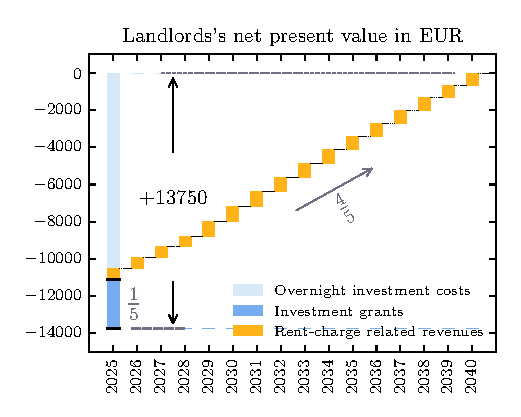
\includegraphics[width=1\linewidth]{figures/3_Methodology/Validate-Landlord.eps}
		\subcaption{Development of landlord's net present value}
		\label{fig:landlord}
	\end{subfigure}
	\begin{subfigure}[c]{0.5\textwidth}
		\centering
		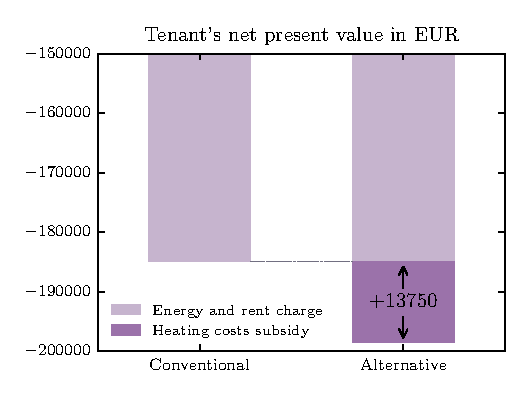
\includegraphics[width=1\linewidth]{figures/3_Methodology/Validate-Tenant.eps}
		\subcaption{Comparison of tenant's net present value}
		\label{fig:tenant}
	\end{subfigure}
	\caption{Landlord's and tenant's net present value and equal financial support. The landlord reaches a net present value equal to zero in 2040 resulting from an investment grant and rent-charge related revenues. The tenant's net present value remains constant compared to the conventional heating system resulting from heating costs subsidy payments.}
	\label{val:npv}
\end{figure}

Both agents receive equal financial support with a total of \SI{13750}{EUR}. One finfth of the landlord's support is paid as an investment grant and four-fifths as rent-charge related revenues. The tenant receives a heating costs subsidy. The level of financial support results exactly in (i) a landlord's net present value equal to zero within the time horizon of 15 years (see Figure \ref{fig:landlord}) and (ii) a constant remaining net present value of tenant compared to the conventional (existing) heating system (including the initial rent charge) (see Figure \ref{fig:tenant}). 

\subsection{Development of an open-source package building on pyam}\label{open}
%The method described will be released as an open-source Python package in the course of publishing this work at the author's GitHub account. In this package, we build on the existing open-source Python package \textit{pyam} \cite{huppmann2021pyam}. \textit{Pyam} is an open-source package for the analysis and visualization of integrated assessment and macro-energy scenarios. In this work, it is used particularly for (i) the linkage between the sequential and the iterative downscaling algorithms, (ii) the internal calculation steps within both downscaling algorithms, and (iii) the visualization of the results. Besides, we used the open-source Python package \textit{networkx} \cite{hagberg2008exploring}, when implementing the iterative downscaling algorithm. We refer to the repository for the codebase, data collection, and further information. 











\newpage
\section{Results and sensitivity analysis}\label{results}
This section presents the most relevant results of the proposed case study. Section \ref{res:overview} compares the results of the district heating or heat-pump-based heat supply in the different scenarios. Section \ref{res:district_heating} puts the focus on the district heating option results in the \textit{Directed Transition} scenario and Section \ref{res:heat_pump} on the implementation of a heat pump system in the \textit{Societal Commitment} scenario. Latter highlights the impact of passive retrofitting measures on the feasibility of the model when implementing a heat pump in the old building and subsidization strategy and presents a sensitivity analysis regarding the total heat demand of the building as a parameter. Finally, Section \ref{res:co2_shares} presents the results in the case of a CO\textsubscript{2} pricing cost allocation between the landlord as the building's owner and the tenants. 

\subsection{Objective value and results comparison}\label{res:overview}
Table \ref{tab:objective} shows a comparison of the obtained objective values for district heating (DH) and heat pump implementation in the different scenarios. 

\definecolor{Gray}{gray}{0.95}
\begin{table}[h]
	\centering
	\resizebox{\columnwidth}{!}{
		\renewcommand{\arraystretch}{1.35}
		\begin{tabular}{lcccccc}
			\toprule 
			& \multicolumn{3}{c}{District heating (DH)} & \multicolumn{3}{c}{Heat pump (HP)}\\
			\cmidrule(lr){2-4}\cmidrule(lr){5-7}
			 & DT & GD & LD & SC & GD& LD\\
			 \cmidrule(lr){2-2}\cmidrule(lr){3-3}\cmidrule(lr){4-4}\cmidrule(lr){5-5}\cmidrule(lr){6-6}\cmidrule(lr){7-7}
			Objective value & (\SI{1.5}{\degreeCelsius}) & (\SI{2.0}{\degreeCelsius}) & (-) & (\SI{1.5}{\degreeCelsius}) &  (\SI{2.0}{\degreeCelsius}) & (-)\\
			\hline
			Absolute in thous. \SI{}{EUR} & \SI{211.4}{} & \SI{195.5}{} & \cellcolor{Gray}\SI{190.1}{} & \textit{infeasible} & \textit{infeasible} & \SI{351.5}{}\\
			Rel. change in \% of LD (DH) & \SI{11.2}{} & \SI{2.6}{} & - &  & & \SI{82.6}{}\\ 
			\bottomrule
	\end{tabular}}
	\caption{Comparison of objective value results for the different heating system alternatives and scenarios}
	\label{tab:objective}
\end{table}

In particular, two important aspects can be obtained while studying this table. The values across the three district heating cases are relatively stable and are within \SI{11.2}{\%}. In addition, the heat pump implementation in the two decarbonization scenarios \textit{Societal Commitment} and \textit{Gradual Development} is infeasible. In this context, only the low CO\textsubscript{2} price development provides a solution for the heat pump but with a significantly higher value compared to the scenario with the lowest value (+\SI{82.6}{\%} compared with the lowest value).\vspace{0.5cm}

Figure \ref{fig:npv_comparison} shows the subsidization from the governance for the different technologies and scenarios. Note that the landlord's rent-related revenues (orange bar) are an implicit subsidy. Hence, the objective values from above are equal to the sum of the tenants' heating costs subsidy (purple bar) and the landlord's investment grant (blue bar). 

\begin{figure}[h]
	\centering
	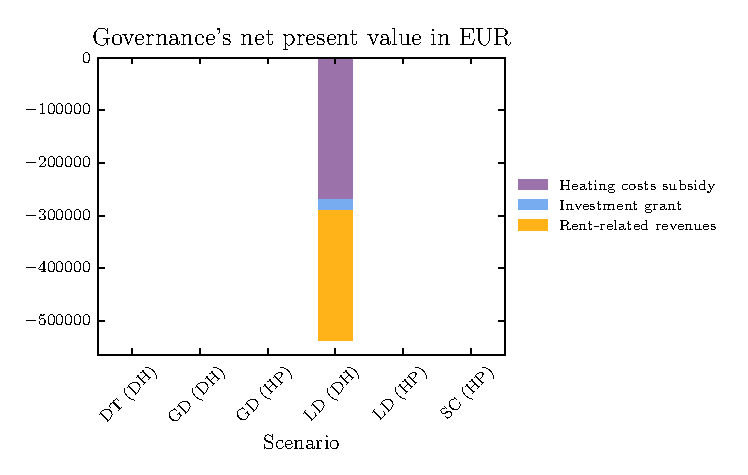
\includegraphics[width=0.7\linewidth]{figures/4_Results/fig_npv_comparison/net_present_value.eps}
	\caption{Comparison of subsidiziation from the governance for the landlord and the tenants for district heating (DH) and heat pump (HP) implementation in the different scenarios}
	\label{fig:npv_comparison}
\end{figure}

\subsection{District heating in the Directed Transition scenario}\label{res:district_heating}
This section presents the results of the district heating implementation in the \textit{Directed Transition} scenario in detail. Figure \ref{fig:dt+dh} shows the revenues and net present value of the landlord and a single tenant within the time horizon $2025$ to $2040$. The subfigure at the top left shows the revenues of the landlord consisting of the overnight investment costs (light blue), investment grant (blue), and rent-related revenues (yellow). Note that later represent the additional rent-related revenues based on the modernization of the building regarding the newly installed sustainable heating system alternative. The subfigure at the bottom left shows the development of the landlord's net present value. Thereby, it is shown that the investment achieves a net present value equal to zero at the end of the time horizon in 2040. The two subfigures to the right illustrate the tenant's revenues (top) and net present value (bottom). The tenant gets subsidy payments from the governance between 2025 and 2030. Thus, the tenant's net present value achieves the same value as in the reference case. The reference case considers constant remaining rent- and heat-related costs for the tenant based on the initial rent, gas, and CO\textsubscript{2} as in 2025. In the years 2025 to 2029, the subsidy payments exceed the heating costs of the tenant. Note that the tenant already pays a higher rent charge to the landlord within the same period (see the yellow bars in the top left subfigure).

\begin{figure}[h]
	\centering
	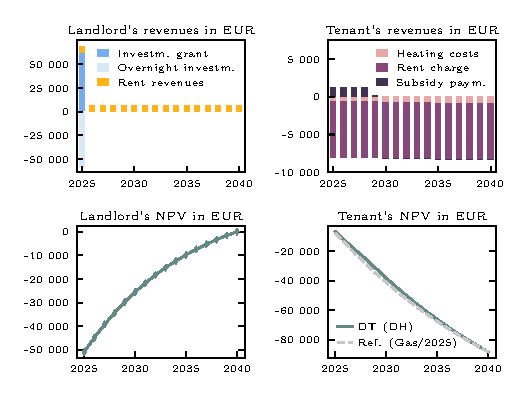
\includegraphics[width=1\linewidth]{figures/4_Results/fig_DT_DH/detail.eps}
	\caption{Development of the landlord's and tenant's economic viability of the district heating option in the \textit{Directed Transition} scenario. Top left: landlord's revenues, bottom left: landlord's net present value (NPV), top right: tenant's revenues, bottom right: tenant's net present value}
	\label{fig:dt+dh}
\end{figure}

Most importantly, the tenant's reference net present value ("Ref. (Gas/2025)" marked by the gray dashed line in the bottom right subfigure) shows a crucial issue of the results and analysis, respectively. Since "Ref. (Gas/2025)" is used as the initial tenant's spendings, the results take into account the fact that the total opportunity costs (hence, those costs that would be incurred by sticking to the initial gas-based heating system for the tenant due to a rising CO\textsubscript{2} price). Note that the decarbonization scenarios do consider both a significant increase of the CO\textsubscript{2} and a decrease of the specific emissions of the district heating and electricity fueling mix. A detailed discussion of the allocation of CO\textsubscript{2} price-related opportunity costs is shown in Section \ref{res:co2_shares}.

\subsection{Heat pump in the Societal Commitment scenario}\label{res:heat_pump}
Figure \ref{fig:retrofitting} shows the results of the heat pump option in the \textit{Societal Commitment} scenario in detail. 

\begin{figure}[h]
	\centering
	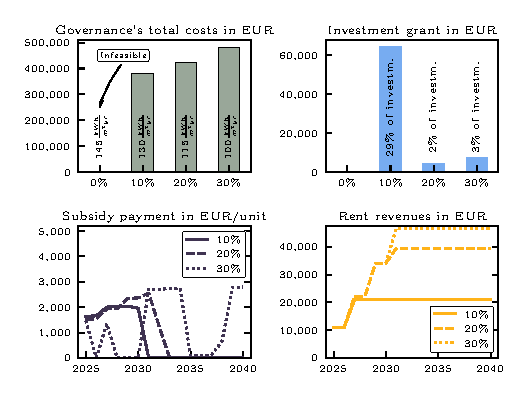
\includegraphics[width=1\linewidth]{figures/4_Results/fig_retrofitting/retrofitting.eps}
	\caption{Comparison of the heat pump option in the \textit{Societal Commitment} scenario for different renovation levels. Top left: governance's objective value, top right: landlord's investment grant, bottom left: tenant's subsidy payment per unit, bottom right: landlord's rent-related revenues in total}
	\label{fig:retrofitting}
\end{figure}

Since the initial condition of the old building in terms of total and peak heat demand leads to the infeasibility of the model, three additional renovation levels are presented. Latter correspond to a \SI{10}{\%}, \SI{20}{\%}, and \SI{30}{\%} reduction of both the total and peak heat demand. The initial condition of the old building is marked by \SI{0}{\%} as no reduction takes place. Most importantly, it can be seen that the building renovation increases the objective value (Fig. \ref{fig:retrofitting} top left). In case of a \SI{10}{\%} reduction of the heat demand, the landlord receives a significant investment grant be equivalent to \SI{29}{\%} of the landlord's total overnight investment costs (Fig. \ref{fig:retrofitting} top right). The tenant's subsidy payment takes place between 2025 and 2030 with a maximum of \SI{2040}{EUR} (Fig. \ref{fig:retrofitting} bottom left). The rent charge adjustment and related revenues remain almost constant during the period (Fig. \ref{fig:retrofitting} bottom right). In case of a \SI{20}{\%} reduction of the heat demand, the landlord receives only a small investment grant related to the total overnight investment costs (around \SI{2}{\%}). The tenant's subsidy payment takes place between 2025 and 2032 with a maximum of approximately \SI{2556}{EUR}. The landlord's rent-related revenues increase until 2031 and then remain constant. In case of a \SI{30}{\%} reduction of the heat demand, the landlord receives as before a small investment grant (\SI{3}{\%} of total overnight investment costs). Instead, the landlord makes significant rent-related revenues (the highest among the three renovation levels). The tenant gets subsidy payments in most years, excluding 2026 and 2028 to 2030. The maximum is \SI{2796}{EUR} in 2040. The lower heat energy-related costs as a result of the building renovation lead to higher rent charge payments. Hence, smaller investment grants supporting the landlord are needed. 

\subsection{Allocation of CO\textsubscript{2} pricing related costs between the governance, landlord and tenant}\label{res:co2_shares}

\definecolor{Gray}{gray}{0.95}
\begin{table}[h]
	\centering
		\renewcommand{\arraystretch}{1.35}
		\begin{tabular}{lccc}
			\toprule
			& \multicolumn{3}{c}{Opportunity costs}\\
			\cmidrule(lr){2-4}
			Rel. allocation among agents& Governance & Landlord & Tenants\\
			\hline
			Case A (all) & \SI{33}{\%} & \SI{33}{\%} & \SI{33}{\%}\\
			Case B (building) & 0 & \SI{50}{\%} & \SI{50}{\%}\\
			Case C (landlord) & 0 & \SI{100}{\%} & 0\\
			Case D (tenant) & \SI{50}{\%} & 0 & \SI{50}{\%}\\
			\hline
			\cellcolor{Gray}Scenarios from Sec. \ref{sec:scenarios} & \cellcolor{Gray}\SI{100}{\%} & \cellcolor{Gray}0 & \cellcolor{Gray}0\\
			\bottomrule
	\end{tabular}
	\caption{}
	\label{tab:allocation}
\end{table}


\section{Conclusions and recommendations}\label{conclusions}
Rapid and equitable decarbonization of the building heat sector is an indispensable cornerstone in a sustainable society. Special attention is needed for the rented residential buildings sector since a sustainable investment decision is in the landlord's hands. Simultaneously, an expected increase in the CO\textsubscript{2} price primarily impacts the tenant's energy costs. This work studies cost-optimal federal subsidy payment strategies incentivizing sustainable heat change and retrofitting measures at the multi-apartment building level. We analyze the results of a the application of the developed modeling framework to a partly renovated old building connecting to the district heating network and implementing an air-sourced heat pump system under several decarbonization storylines.\vspace{0.5cm}

We found that a fair sustainable heat system change is possible but with massive federal subsidy payments. In particular, the building's owner investment grant and additional rent-related revenues based on the building modernization are crucial to trigger the profitability of the investment. At the same time, subsidy payments are required at the beginning of the investment period to limit the energy and rent-related spendings of the tenants. Furthermore, the results imply that the heat pump alternative is not competitive in supplying heat service needs in partly renovated old buildings. Either the subsidy payments are significantly higher than in the district heating case, or the equitable constraints of the model can not be satisfied. Building renovation and reducing heat demand lead to feasibility but with high total costs because passive retrofitting measures need to be incentivized.\vspace{0.5cm}

Moreover, the results demonstrate that allocating the costs of inaction between the governance, the building owner, and the tenants is an important lever and can reduce the required subsidy payments. First and foremost, the biggest drop of the objective value (to nearly half) takes place when the costs of inaction are completely borne by the building owner. Also, a decrease in the landlord's interest rate reduces the total costs but limits the maximum share of the costs of inaction allocated to the landlord and implies a lower bound of the cost-minimized solution.\vspace{0.5cm}

Future work may investigate a stronger coupling of active and passive renovation measures as a necessary condition for federal subsidy payments. This could bring further insights to decarbonization strategies with an eye on the heat demand and sustainable heat source alternatives in the residential building sector (i.e., climate neutrality in 2050). Besides, the tenant's set-up of the building could be improved. In particular, further work should include different types of tenants within the building (e.g., different willingness to pay). More generally, this study could be extended by introducing further technology options, such as solar photovoltaic, solar thermal, and heat and electricity storage systems. 

\section*{Declaration of interests}
None.
\section*{Declaration of Competing Interest}
The authors report no declarations of interest.
\section*{Acknowledgments}
This project has received funding from the European Union's Horizon 2020 Research and Innovation Programme under Grant Agreement No. 835896. The authors acknowledge TU Wien Bibliothek for financial support through its Open Access Funding Programme.

\bibliography{mybibfile}
\appendix
\setcounter{table}{0}
\setcounter{figure}{0}
\section{Data}\label{app:data}
\begin{table}[h]
	\centering
	\scalebox{0.85}{
		\renewcommand{\arraystretch}{1.35}
		\begin{tabular}{llr}
			\toprule 
			Variable & Unit & Value\\\hline
			Specific emissions$\vert$Electricity & \SI{}{kgCO_{2} \per kWh} & \SI{0.130}{}\\
			Specific emissions$\vert$District heating & \SI{}{kgCO_{2} \per kWh} & \SI{0.130}{}\\
			Specific emissions$\vert$Natural gas & \SI{}{kgCO_{2} \per kWh} & \SI{0.220}{}\\
			Price$\vert$District heating & \SI{}{EUR \per kWh} & \SI{0.047}{}\\
			Price$\vert$Natural gas & \SI{}{EUR \per kWh} & \SI{0.05}{}\\
			Price$\vert$Electricity & \SI{}{EUR \per kWh} & \SI{0.2}{}\\
			Coefficient of performance (heat pump) & \SI{}{1} & \SI{3}{}\\
			\bottomrule
	\end{tabular}}
	\caption{2020's economic parameters and empirical settings}
	\label{tab:a1}
\end{table}

\section{Empirical settings of the small case example}\label{app:verify}
\begin{table}[h]
	\centering
	\scalebox{0.85}{
		\renewcommand{\arraystretch}{1.35}
		\begin{tabular}{llr}
			\toprule 
			Variable & Unit & Value\\\hline
			Heat pump investment costs & \SI{}{EUR \per kW} & \SI{1000}{}\\
			Construction costs & \SI{}{EUR} & \SI{1000}{}\\
			Initial rent price & \SI{}{EUR \per m^2} & \SI{10}{}\\
			Rented area & \SI{}{m^2} & \SI{100}{}\\	
			Total heat demand & \SI{}{kWh} & \SI{22000}{}\\		
			Peak heat demand & \SI{}{kW} & \SI{13}{}\\	
			CO\textsubscript{2} price (2025-2034) & \SI{}{EUR \per tCO_{2}} & \SI{50}{}\\
			CO\textsubscript{2} price (2035-2040) & \SI{}{EUR \per tCO_{2}} & \SI{100}{}\\
			Natural gas price & \SI{}{EUR \per kWh} & \SI{0.05}{}\\
			Electricty price & \SI{}{EUR \per kWh} & \SI{0.2}{}\\
			Specific emissions$\vert$Electricity & \SI{}{kgCO_{2} \per kWh} & \SI{0.130}{}\\
			\bottomrule
	\end{tabular}}
	\caption{Small case example's parameters}
	\label{tab:a2}
\end{table}
\end{document}